\chapter{Исследовательская часть}

\section{Технические характеристики}

Технические характеристики устройства, на котором выполнялись замеры по времени, представлены далее.

\begin{itemize}
	\item Процессор: AMD Ryzen 5 5500U\,--\,2.10 ГГц;
	\item Оперативная память: 16 ГБайт;
	\item Операционная система: Windows 10 Pro 64-разрядная система версии 22H2.
\end{itemize}

При замерах времени ноутбук был включен в сеть электропитания и был нагружен только системными приложениями.

\section{Демонстрация работы программы}

На рисунке \ref{img:demonstration} представлена демонстрация работы разработанного ПО, а именно показаны результаты работы алгоритмов поиска расстояний Левенштейна и Дамерау~---~Левенштейна на примере двух строк \textit{<<секста>>} и \textit{<<септима>>}.  
\clearpage
\begin{figure}[h]
	\centering
	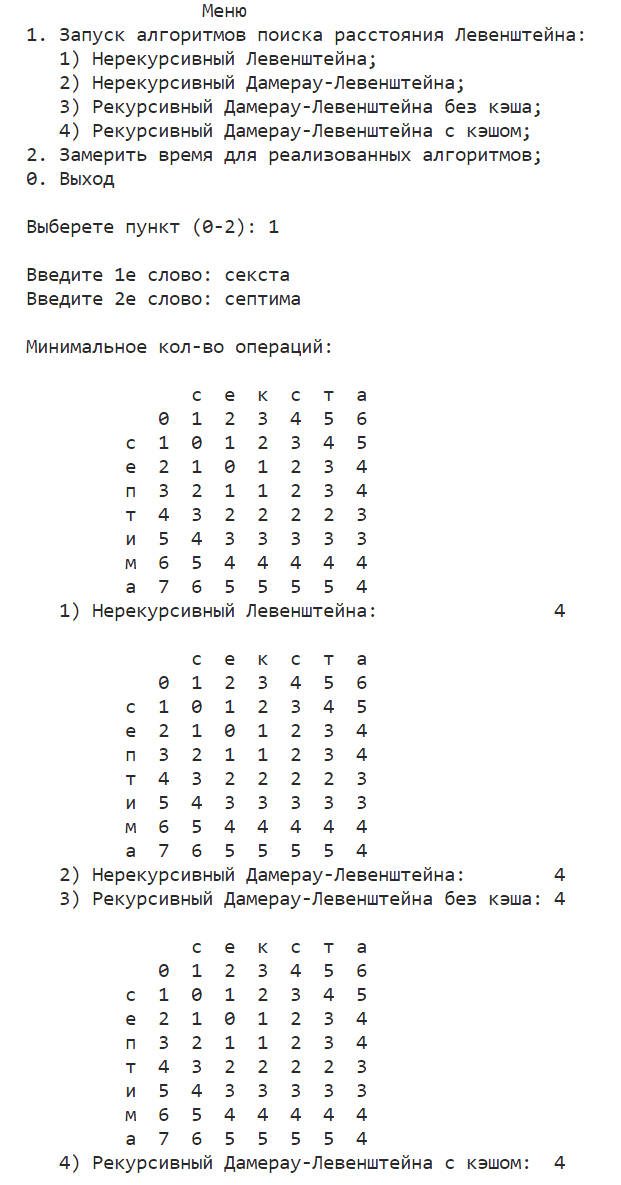
\includegraphics[height=0.7\textheight]{img/prog_work.png}
	\caption{Демонстрация работы программы}
	\label{img:demonstration}
\end{figure}

\clearpage

\section{Временные характеристики}

Все реализации алгоритмов сравнивались на случайно сгенерированных строках длиной:
\begin{itemize}
	\item 0--10 с шагом 1 для всех алгоритмов;
	\item 10--200 с шагом 10 для нерекурсивных и рекурсивного с кешированием. 
\end{itemize}

Поскольку замеры по времени имеют некоторую погрешность, для каждой строки и каждой реализации алгоритма замеры производились 1000 раз, а затем вычислялось среднее арифметическое значение.

На рисунке \ref{plt:time_01} представлен график, иллюстрирующий зависимость времени работы от длины строк для рекурсивных реализаций алгоритмов поиска расстояния Дамерау~---~Левенштейна с кешем и без.
\begin{figure}[H]
	\centering
	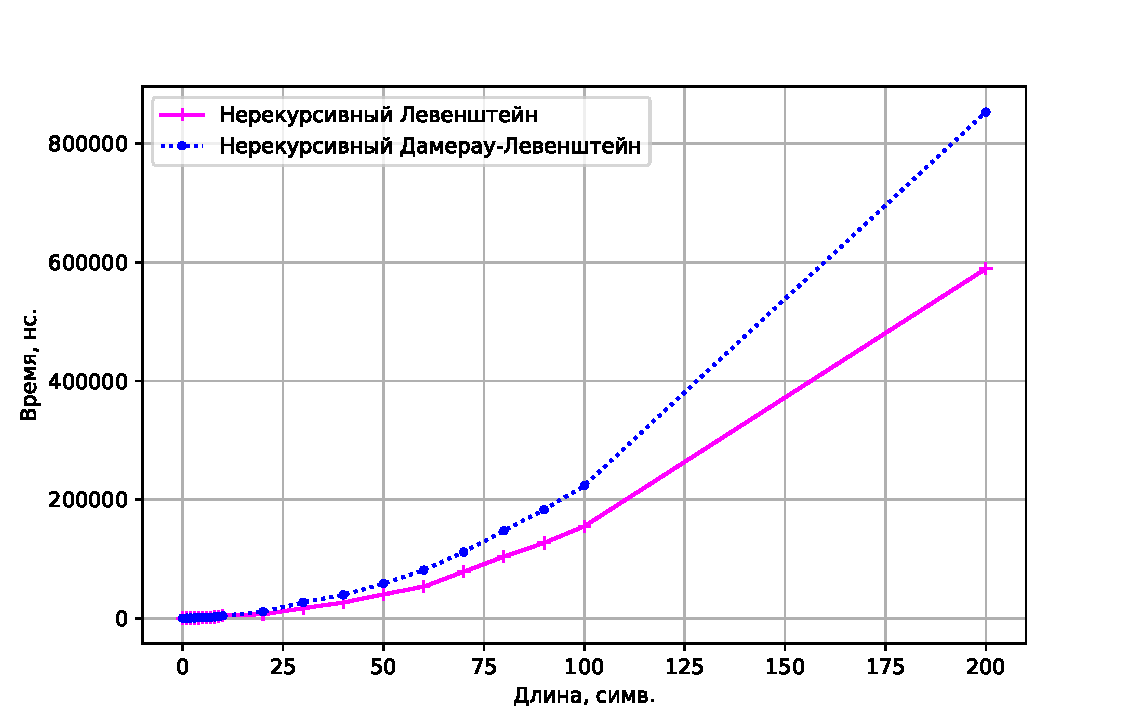
\includegraphics[height=0.5\textheight, page=1]{img/figures.pdf}
	\caption{Сравнение по времени рекурсивных реализаций алгоритмов поиска расстояния Дамерау~---~Левенштейна с кешем и без}
	\label{plt:time_01}
\end{figure}

На рисунке \ref{plt:time_02} представлен график, иллюстрирующий зависимость времени работы от длины строк для итеративных реализаций алгоритмов поиска расстояний Левенштейна и Дамерау~---~Левенштейна.
\begin{figure}[H]
	\centering
	\includegraphics[height=0.5\textheight, page=2]{img/figures.pdf}
	\caption{Сравнение по времени итеративных реализаций алгоритмов поиска расстояний Левенштейна и Дамерау~---~Левенштейна}
	\label{plt:time_02}
\end{figure}

На рисунке \ref{plt:time_03} представлен график, иллюстрирующий зависимость времени работы от длины строк для итеративной реализации и рекурсивной реализации с использованием кеша алгоритма поиска расстояния Дамерау~---~Левенштейна. 
\begin{figure}[H]
	\centering
	\includegraphics[height=0.5\textheight, page=3]{img/figures.pdf}
	\caption{Сравнение по времени итеративной реализации и рекурсивной реализации с использованием кеша алгоритма поиска расстояния Дамерау~---~Левенштейна}
	\label{plt:time_03}
\end{figure}

\section{Характеристики по памяти}

Введем следующие обозначения:
\begin{itemize}
	\item$n$~--- длина строки $S_{1}$;
	\item$m$~--- длина строки $S_{2}$;
	\item$size()$~--- функция вычисляющая размер в байтах;
	\item $char$~--- тип, используемый для хранения символа строки;
	\item $int$~--- целочисленный тип.
\end{itemize}

Использование памяти при \textbf{итеративной реализации} алгоритма поиска расстояния Левенштейна теоретически равно:
\begin{equation}
	\label{eq:lev_mtr_memory}
	\begin{aligned}
		M_{iter} = (m + 1) \cdot (n + 1) \cdot size(int) + (n + m) \cdot size(char) + \\ + 5 \cdot size(int) + size(int **) + (n + 1) \cdot size(int *),
	\end{aligned}
\end{equation}
где $(n + 1) \cdot (m + 1) \cdot size(int)$~--- хранение матрицы;
\newline $(n + m) \cdot size(char)$~--- хранение двух строк;
\newline $2 \cdot size(int)$~--- хранение размеров строк;
\newline $3 \cdot size(int)$~--- дополнительные переменные;
\newline $size(int**) + (n + 1) \cdot size(int *)$~--- указатель на матрицу.

Использование памяти при \textbf{итеративной реализации} алгоритма поиска расстояния Дамерау~---~Левенштейна идентично формуле (\ref{eq:lev_mtr_memory}).

Рассчитаем затраты по памяти для \textbf{рекурсивного} алгоритма поиска расстояния Дамерау~---~Левенштейна\textit{ (для каждого вызова)}:
\begin{equation}
	\begin{aligned}
		M_{call} = (m + n) \cdot size(char) + 4 \cdot size(int) + 8 байт,
	\end{aligned}
\end{equation}
где $(n + m) \cdot size(char)$~--- хранение двух строк;
\newline $2 \cdot size(int)$~--- хранение размеров строк;
\newline $2 \cdot size(int)$~--- дополнительные переменные;
\newline 8 байт~--- адрес возврата.

Макисмальная глубина стека вызовов при рекурсивной реализации равна сумме длин входящий строк, поэтому макисмальный расход памяти равен:
\begin{equation}
	\begin{aligned}
		M_{rec} = (n + m) \cdot M_{call},
	\end{aligned}
\end{equation}
где $n + m$~--- максимальная глубина стека;
\newline $M_{call}$~--- затраты по памяти для одного рекурсивного вызова.

Для рекурсивного алгоритма поиска расстояния Дамерау~---~Левенштейна с использованием кеша необходимо подсчитать размер самого кеша:
\begin{multline}
	M_{cash} = (m + 1) \cdot (n + 1) \cdot size(int) + \\ + size(int **) + (n + 1) \cdot size(int *),
\end{multline}
где $(m + 1) \cdot (n + 1)$~--- количество элементов в кеше;
\newline $size(int **) + (n + 1) \cdot size(int *)$~--- хранение указателей.

Затраты по памяти для рекурсивного алгоритма поиска расстояния Дамерау~---~Левенштейна с учетом кеша: 
\begin{equation}
	\label{}
	\begin{aligned}
		M_{recCash} = M_{rec} + M_{cash}.
	\end{aligned}
\end{equation}

\section{Вывод}

По времени выполнения:
\begin{enumerate}
	\item при малых длинах строк $(< 5)$ рекурсивные реализации с кешем и без для поиска расстояния Дамерау~---~Левенштейна имеют приблизительно одинаковое время работы, 
	но с увеличением длины строки реализация без кеша выполняется на порядок дольше, поскольу не происходит повторное вычисление значений (см рис. \ref{plt:time_01});
	\item разница между итеративными реализацими алгоритмов поиска расстояний Левенштейна и Дамерау~---~Левенштейна незначительна, и обусловлена она
	дополнительным условием на проверку равенства соседних символов для расстояния Дамерау~---~Левенштейна (см рис. \ref{plt:time_02});
	\item итеративная реализация работает на порядок быстрее рекурсивной с кешем для поиска расстояния Дамерау~---~Левенштейна (см рис. \ref{plt:time_03}).
\end{enumerate}

Проанализировав использование памяти в алгоритмах, можно сделать вывод, что итеративные алгоритмы и рекурсивные алгоритмы с кешированием требуют больше памяти по сравнению с рекурсивным алгоритмом без кеширования. 
В реализациях, использующих матрицы, максимальный используемый объем памяти увеличивается пропорционально произведению длин строк. С другой стороны, для рекурсивного алгоритма без кеширования потребление памяти 
увеличивается пропорционально сумме длин строк.